\documentclass[10pt]{article} 
\usepackage[spanish,activeacute]{babel} %idioma español
\usepackage[utf8]{inputenc}             %transforma los tildes a lenguaje latex automáticamente
\usepackage{multirow}                   %Permite cosntruir tablas en las que algunas celdas ocupan varias filas dentro de un entorno tabular con la orden \multirow, en el caso de columnas es \multicolumn  ... \multirrow{nrow}{width}[vmove]{contenido}
% nrow: número de filas a agrupar
%width: ancho de la columna
%vmove: sirve para subir o bajar el texto (opcional)
\usepackage{epsfig}                     %permite incluir gráficos eps
\usepackage{graphicx}                   %Permite incluir gráficos e imágenes
\usepackage{subfig}                     %Permite hacer subfiguras
\usepackage{amsmath}                    %Extiende el modo matemático
\usepackage{amsthm}
\usepackage{amssymb}
\usepackage{mathrsfs}
\usepackage{hyperref}
\usepackage{colortbl} %Permite agregar color a las tablas
\usepackage{epstopdf}                 %Permite utilizar imagenes en formato eps
\usepackage{float}   %permite indicar la posición de las figuras
\usepackage[left=3cm,right=3cm,top=3cm,bottom=3cm]{geometry}
\renewcommand{\baselinestretch}{1.5}
\parskip=4pt

\usepackage{fullpage}            %%
\usepackage{fancyhdr} 
\usepackage{mdframed}            %%

\setlength{\headheight}{54pt}    %%
\setlength{\headsep}{1em}        %%
\setlength{\textheight}{8.5in}  
\setlength{\footskip}{0.5in} 


\fancypagestyle{firstpage}
{
  \fancyhf{}
  \lhead{
\includegraphics[height=5em]{LogoDFI.jpg}}
  \rhead{FI3104-1 \semestre\\
         Métodos Numéricos para la Ciencia e Ingeniería\\
         Prof.: \profesor}
  \fancyfoot[C]{\thepage}
}

\pagestyle{plain}
\fancyhf{}
\fancyfoot[C]{\thepage}


\newcommand{\semestre}{2016-2}
\newcommand{\profesor}{Valentino González}



\begin{document}

\author{Sergio Leiva M.}
\title{\textbf{Informe Tarea 11}}
\date{}
\maketitle

\thispagestyle{firstpage}


\section{Introducción}
Las ecuaciones de \textit{Fisher-KPP} (\ref{ec_enunciado_1}) en 1D y \textit{Newell-Whitehead-Segel}(\ref{ec_enunciado_2}), y son llamadas ecuaciones de reacción-difusión. La ecuación \ref{ec_enunciado_1} busca modelar el comportamiento de una especie animal, donde la variable $n=n(t,x)$ describe la densidad de la especia como función del tiempo y la posición. Pero la ecuación (\ref{ec_enunciado_2}) describe fenómenos de convección y combustión entre otros.

\begin{equation}
\frac{\partial n}{\partial t} =
\gamma \frac{\partial^2n}{\partial x^2} + \mu n - \mu n^2
\label{ec_enunciado_1}
\end{equation}
\begin{equation}
\frac{\partial n}{\partial t} =
\gamma \frac{\partial^2n}{\partial x^2} + \mu (n - n^3)
\label{ec_enunciado_2}
\end{equation}
 
Para esta tarea se pidio resolver las ecuaciones (\ref{ec_enunciado_1}) y (\ref{ec_enunciado_2}), usando el método de \textit{Crank-Nicolson}(\ref{ec_C_N}) para la parte de difusión y el método de Euler explícito (\ref{ec_E_expl}) para la parte  de reacción, en ambas ecuaciones. Tomando valores como se muestran en el Cuadro \ref{tab_valores} y para el primer caso, con las condiciones de borde :

\begin{flalign*} 
  n(t, 0) &= 1\\
  n(t, 1) &= 0\\
  n(0, x) &= e^{-x^2/0.1}
\end{flalign*}

En el caso del segundo caso:

\begin{flalign*}
  n(t, 0) &= 0\\
  n(t, 1) &= 0\\
  n(0, x) &= \texttt{np.random.uniform(low=-0.3, high=0.3, size=Nx)} 
\end{flalign*}
 
\begin{equation}
\frac{u_{i}^{n + 1} - u_{i}^{n}}{\Delta t} =
\frac{1}{2}\left[
F_{i}^{n + 1}\left(u, x, t, \frac{\partial u}{\partial x}, \frac{\partial^2 u}{\partial x^2}\right) + 
F_{i}^{n}\left(u, x, t, \frac{\partial u}{\partial x}, \frac{\partial^2 u}{\partial x^2}\right)
\right] \qquad \mbox{(Crank-Nicolson)}
\label{ec_C_N}
\end{equation}
  
 
\begin{equation}
\frac{u_{i}^{n + 1} - u_{i}^{n}}{\Delta t} = 
F_{i}^{n}\left(u, x, t, \frac{\partial u}{\partial x}, \frac{\partial^2 u}{\partial x^2}\right) \qquad \mbox{(Euler explícito)}
\label{ec_E_expl}
\end{equation} 

En las expresiones anteriores para los métodos de \textit{Crank-Nicolson} y \textit{Euler explícito} usamos el paso espacial ($\Delta x$) y el paso temporal ($\Delta t$) para discretizar las derivadas patciales, espaciales y temporales.

\begin{table}
\centering
\begin{tabular}{|c|c|}
\hline
Constante & Valor \\
\hline
$\gamma$ & 0.001 \\
\hline
$\mu$ & 1.5 \\
\hline
 t & 4 \\
\hline
\end{tabular}
\caption{Cuadro de constantes de la ecuación \ref{ec_enunciado_1} y \ref{ec_enunciado_2}, además el término t, hace referencia al tiempo final hasta el que se integró.}
\label{tab_valores}
\end{table}

\section{Procedimiento}
  Al implementar los métodos \ref{ec_C_N} y \ref{ec_E_expl} para las ecuaciones que se piden resolver, y usando $r = \frac{\gamma \Delta t}{2 (\Delta x)^2}$ vemos que las ecuaciones discretizadas, despues de un poco de trabajo algebraico nos quedan de la forma:
 $$-r n_{x + 1}^{t + 1} + (1 + 2 r)n_{x}^{t + 1} - r n_{x - 1}^{t + 1} = r n_{x + 1}^{t} + (1 - 2 r)n_{x}^{t} + r n_{x - 1}^{t} +\mu (n_{x}^{t} -(n_{x}^{t})^2)$$

 $$-r n_{x + 1}^{t + 1} + (1 + 2 r)n_{x}^{t + 1} - r n_{x - 1}^{t + 1} = r n_{x + 1}^{t} + (1 - 2 r)n_{x}^{t} + r n_{x - 1}^{t} +\mu (n_{x}^{t} -(n_{x}^{t})^3)$$
 
 Además al evaluar puntos de equilibrio , vemos que para la primera ecuación tiene dos puntos de equilibrio $n = 0$ y $n = 1$, pero sólo el segundo es estable y la segunda tiene 3 puntos de equilibrio, $n = 0$ (inestable) y $n = \pm1$ (estables). En el último caso vemos que para cada valor posible siempre tiende al valor 1, estable.
 
Para resolver este problema, nos planteamos una matriz n, que tenga en que las columnas representan una posición y las filas un tiempo. Por lo que para resolver estos sistemas, vemos que el lado izquierdo es igual y depende de la fila siguiente (t+1), y el lado derecho depende de la fila actual (t), por lo que cada fila solo depende de la anterior. Dada la estructura de las condiciones iniciales (la primera fila es dato), vemos que el lado derecho resulta ser dato en cada paso que ya tenga resuelto el caso anterior por lo que nos proponemos resolver un sistema lineal tipo $ A\vec{a} = \vec{b} $, con $\vec{a}$ la fila (t+1) de la matriz n, y A la matriz que contiene a los factores para hacer el sistema de ecuaciones. A esta matriz se le debe imponer las condiciones de borde respectivas.

 Con lo anterior listo, se pudo resolver la fila (t+1) a partir de la fila t, y dado que la fila (0) es dato inicial, basto con resolver sistematicamente desde la fila 0 a la última. Es importante notar que usando esta implementación y funciones modulares, los desarrollos difieren en las condiciones iniciales y de borde, además de los términos $n^2$ y $n^3$. 

\section{Resultados}
Para el caso de la ecuación \ref{ec_enunciado_1} vemos que al avanzar en el tiempo la solución tiende al punto estable, ($n = 1$) y además se ve como al disminuir el dt (paso temporal), el algoritmo pasa a ser mas suave y una mejor aproximación.

\begin{figure}[H]
\centering
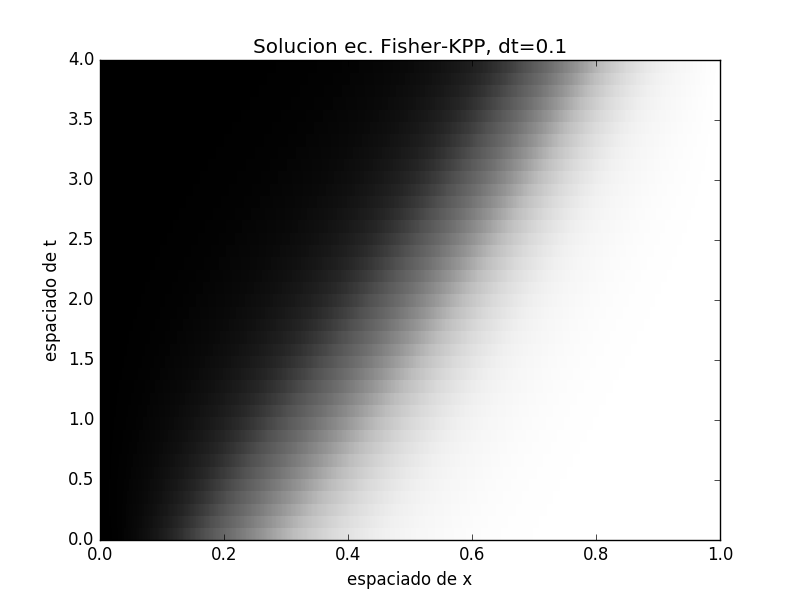
\includegraphics[scale=0.4]{imgp1_01.png}
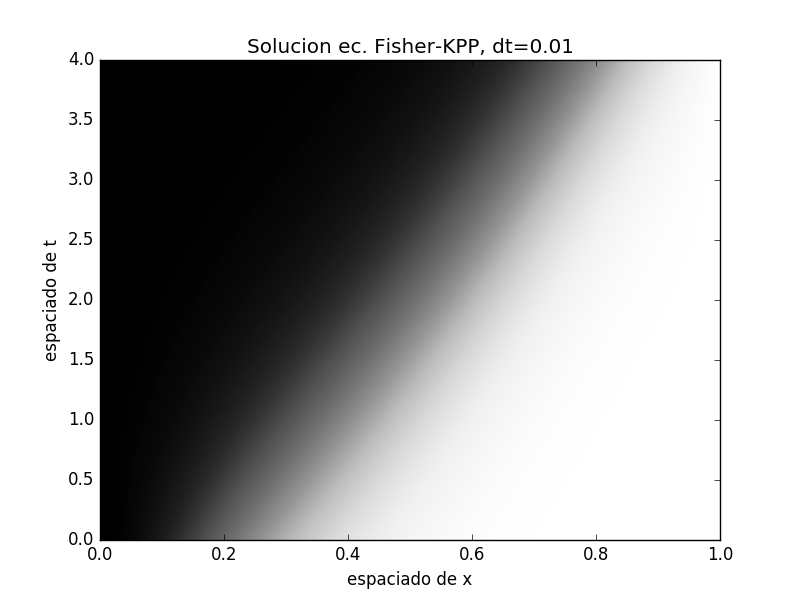
\includegraphics[scale=0.4]{figure_1_001.png}
\end{figure}

El segundo caso, mostró que al tomar valores aleatorios en [-0.3,0.3], se vio que converge a los puntos de equilibrio, al ir aumentando el tiempo. 

\begin{figure}[H]
\centering
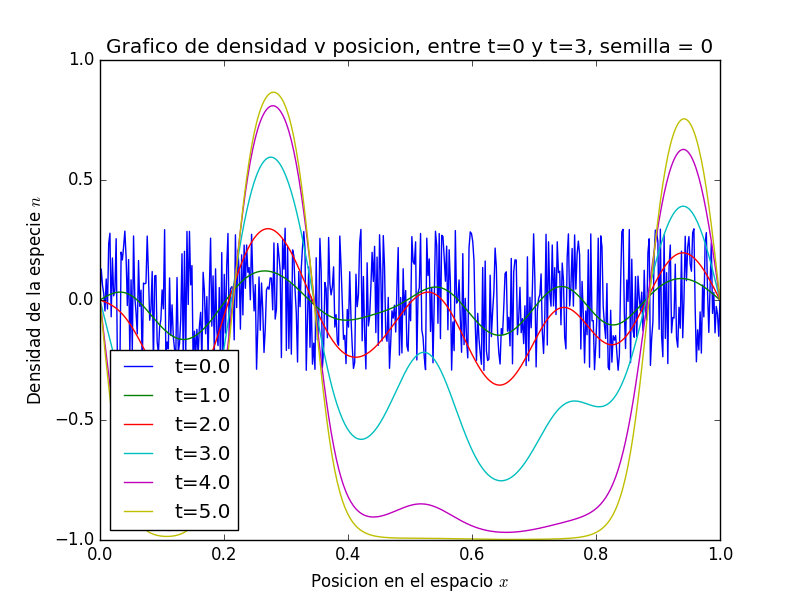
\includegraphics[scale=0.3]{p_2_0.png}
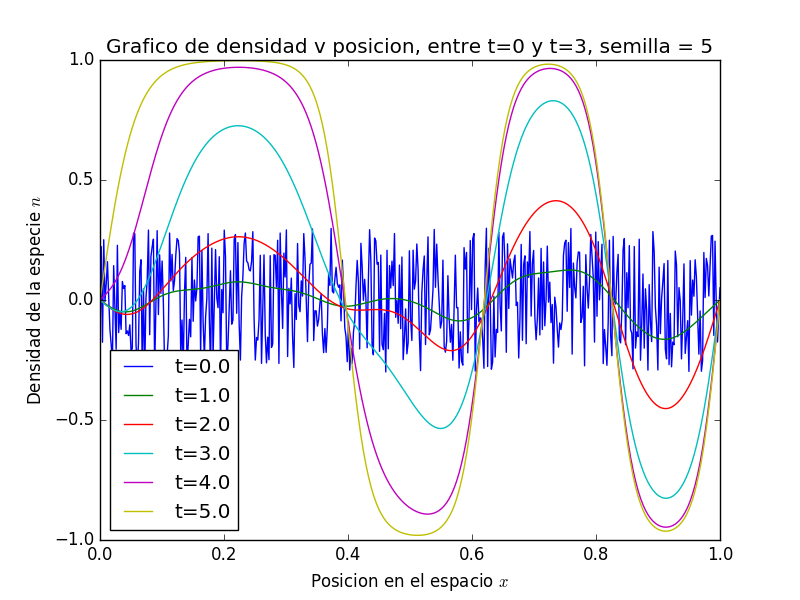
\includegraphics[scale=0.3]{p_2_5.png}
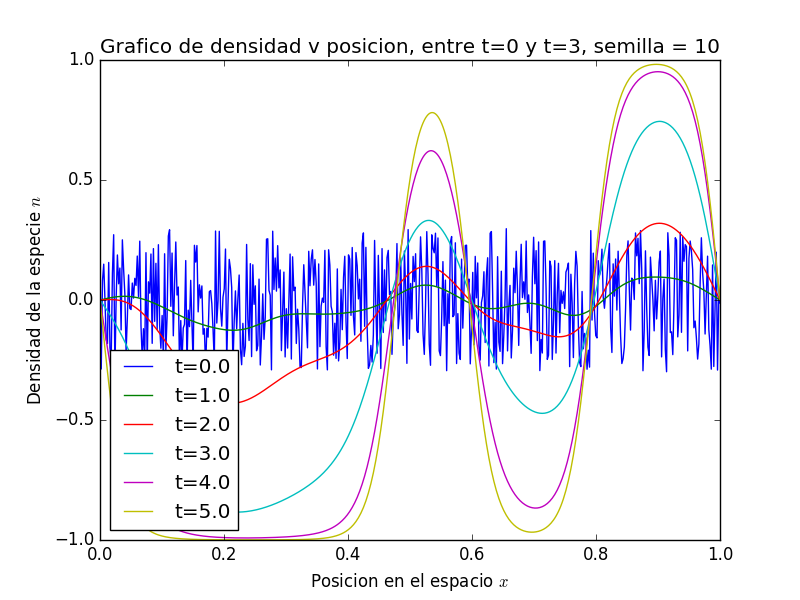
\includegraphics[scale=0.3]{p_2_10.png}
\end{figure}

\begin{figure}[H]
\centering
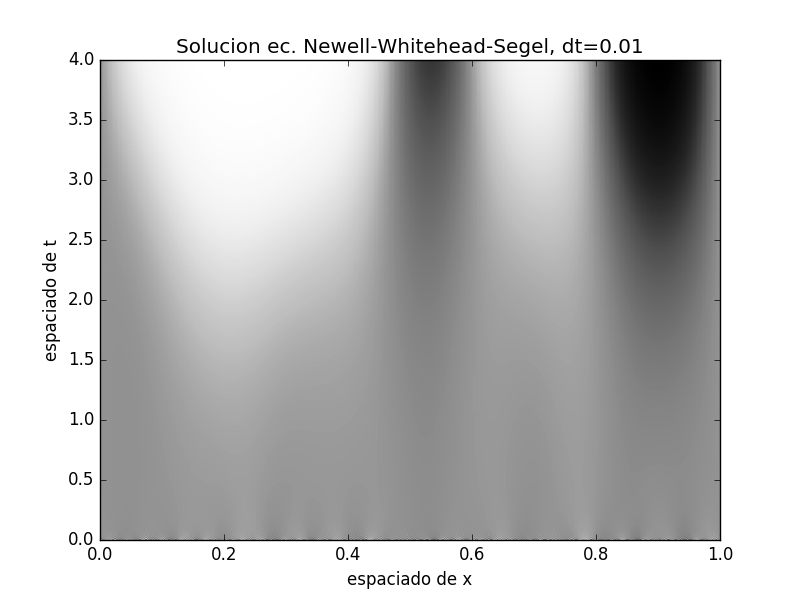
\includegraphics[scale=0.35]{figure_p2_0.png}

\end{figure}



\section{Conclusiones}
 Se vio que al variar la relación entre los paso temporal y espacial, la solución convergia de mejor o peor. Pero siempre mantuvo una solución notoria, para el primer caso vemos media gaussiana, pero que al pasar el tiempo no se completa sino que se aproxima al valor 1. 
 Para el caso 2, se ve que aun siendo aleatoria la condición de borde, esta converge a los puntos de equilibrio.  En la imagen de escala de grises(semilla=10) de la solución para la ecuación de Newell-Whitehead-Segel, se ve que al llegar a los valores máximos del tiempo, la solución converge a puntos extremos, asi como muestran las imagenes con diferentes semillas.

\end{document}}